%% This Beamer template is based on the one found here: https://github.com/sanhacheong/stanford-beamer-presentation, and edited to be used for Stanford ARM Lab

\documentclass[12pt]{beamer}
\usetheme{Frankfurt}
%\usecolortheme{beaver}
%\mode<presentation>{}
\usepackage{amssymb,amsmath,amsthm,enumerate}
\usepackage[utf8]{inputenc}
\usepackage{array}
\usepackage[parfill]{parskip}
\usepackage{graphicx}
\usepackage{caption}
\usepackage{subcaption}
\usepackage{bm}
\usepackage{amsfonts,amscd}
\usepackage[]{units}
\usepackage{listings}
\usepackage{multicol}
\usepackage{multirow}
\usepackage{tcolorbox}
\usepackage{physics}
\usepackage{xcolor}
\usepackage{hyperref}
\usepackage{tikz}
\usetikzlibrary{positioning, shapes.geometric}
% Enable colored hyperlinks
\hypersetup{colorlinks=true}

% The following three lines are for crossmarks & checkmarks
\usepackage{pifont}% http://ctan.org/pkg/pifont
\newcommand{\cmark}{\ding{51}}%
\newcommand{\xmark}{\ding{55}}%

% Numbered captions of tables, pictures, etc.
\setbeamertemplate{caption}[numbered]

%\usepackage[superscript,biblabel]{cite}
\usepackage{algorithm2e}
\renewcommand{\thealgocf}{}

% Bibliography settings
\usepackage[style=apa]{biblatex}
\setbeamertemplate{bibliography item}{\insertbiblabel}
\addbibresource{references/rq1.bib}
\addbibresource{references/rq2.bib}
\addbibresource{references/rq3.bib}
\addbibresource{references/rq4.bib}
\addbibresource{references/rq5.bib}
\addbibresource{references/methodology.bib}
\addbibresource{references/others.bib}
%\addbibresource{references/references.bib}
% Glossary entries
\usepackage[acronym]{glossaries}
\newacronym{ML}{ML}{machine learning}
\newacronym{HRI}{HRI}{human-robot interactions}
\newacronym{RNN}{RNN}{Recurrent Neural Network}
\newacronym{LSTM}{LSTM}{Long Short-Term Memory}


\theoremstyle{remark}
\newtheorem*{remark}{Remark}
\theoremstyle{definition}

\newcommand{\empy}[1]{{\color{darkorange}\emph{#1}}}
\newcommand{\empr}[1]{{\color{cardinalred}\emph{#1}}}
\newcommand{\examplebox}[2]{
\begin{tcolorbox}[colframe=darkcardinal,colback=boxgray,title=#1]
#2
\end{tcolorbox}}

%\usetheme{default} 
%\def \i  {\item}
\def \ai {\item[] \quad \arrowbullet}
\newcommand \si[1]{\item[] \quad \bulletcolor{#1}}
\def \wi {\item[] \quad $\ \phantom{\Rightarrow}\ $}
\def \bi {\begin{itemize}\item}
\def \ei {\end{itemize}}
\def \be {\begin{equation*}}
\def \ee {\end{equation*}}
\def \bie {$\displaystyle{}
\def \eie {{\ }$}}
\def \bsie {\small$\displaystyle{}
\def \esie {{\ }$}\normalsize\selectfont}
\def \bse {\small\begin{equation*}}
\def \ese {\end{equation*}\normalsize}
\def \bfe {\footnotesize\begin{equation*}}
\def \efe {\end{equation*}\normalsize}
\renewcommand \le[1] {\\ \medskip \lefteqn{\hspace{1cm}#1} \medskip}
\def \bex {\begin{example}}
\def \eex {\end{example}}
\def \bfig {\begin{figure}}
\def \efig {\end{figure}}
\def \btheo {\begin{theorem}}
\def \etheo {\end{theorem}}
\def \bc {\begin{columns}}
\def \ec {\end{columns}}
\def \btab {\begin{tabbing}}
\def \etab {\end{tabbing}\svneg\svneg}
\newcommand \col[1]{\column{#1\linewidth}}
\def\vneg  {\vspace{-5mm}}
\def\lvneg {\vspace{-10mm}}
\def\svneg {\vspace{-2mm}}
\def\tvneg {\vspace{-1mm}}
\def\vpos  {\vspace{5mm}}
\def\lvpos {\vspace{10mm}}
\def\svpos {\vspace{2mm}}
\def\tvpos {\vspace{1mm}}
\def\hneg  {\hspace{-5mm}}
\def\lhneg {\hspace{-10mm}}
\def\shneg {\hspace{-2mm}}
\def\thneg {\hspace{-1mm}}
\def\hpos  {\hspace{5mm}}
\def\lhpos {\hspace{10mm}}
\def\shpos {\hspace{2mm}}


%\logo{
\includegraphics[height=0.4in]{images/univalle.png}}

% commands to relax beamer and subfig conflicts
% see here: https://tex.stackexchange.com/questions/426088/texlive-pretest-2018-beamer-and-subfig-collide
\makeatletter
\let\@@magyar@captionfix\relax
\makeatother

\title[Defense of Research proposal]{Characterizing and understanding security risks through Security-Aware Mutation Testing of security configuration in RESTful APIs}
%\subtitle{Subtitle Of Presentation}

%\beamertemplatenavigationsymbolsempty
\AtBeginSection[]{
  \begin{frame}
  \vfill
  \centering
  \begin{beamercolorbox}[sep=8pt,center,shadow=true,rounded=true]{title}
    \usebeamerfont{title}\insertsectionhead\par%
  \end{beamercolorbox}
  \vfill
  \end{frame}
}

\DeclareUnicodeCharacter{0301}{\'{e}}

\author[Carlos Delgado]{
    \normalsize{Carlos Andres Delgado Saavedra}\\
    \footnotesize \href{mailto:carlos.andres.delgado@correounivalle.edu.co}{carlos.andres.delgado@correounivalle.edu.co} \\ 
    Advisors:\\
    Jesus A. Aranda, PhD. Universidad del Valle \\
    Gills Perrouin, PhD. Universite de Namur \\
    James Ortiz. PhD, Universite de Namur
    }

\usepackage{tikz}
\usetikzlibrary{shapes.geometric, arrows, positioning}


\begin{document}

\institute{
	\vskip 5pt
	\begin{figure}
		\centering
		\begin{subfigure}[t]{0.33\textwidth}
			\centering
			
\includegraphics[height=0.4in]{images/univalle.png}
		\end{subfigure}%
		\begin{subfigure}[t]{0.33\textwidth}
			\centering
			
\includegraphics[height=0.4in]{images/logounamur.png}
		\end{subfigure}%
		~ 
		\begin{subfigure}[t]{0.33\textwidth}
			\centering
			
\includegraphics[height=0.4in]{images/avispalogo.png}
		\end{subfigure}
	\end{figure}
	\vskip 5pt
	%Escuela de Ingenieria de Sistemas y Computacion\\
	%Universidad del Valle\\
	%Colombia
	\vskip 3pt
}

\date{December, 2024}


\begin{frame}[plain]\maketitle\end{frame}


\setbeamertemplate{itemize items}[default]
\setbeamertemplate{itemize subitem}[circle]

\begin{frame}
	\frametitle{Overview} % Table of contents slide, comment this block out to remove it
	\tableofcontents % Throughout your presentation, if you choose to use \section{} and \subsection{} commands, these will automatically be printed on this slide as an overview of your presentation
\end{frame}

\section{Introduction}
\begin{frame}[allowframebreaks]
\frametitle{Introduction}
\begin{block}{Background}
RESTful APIs are essential for enabling communication between web applications and services, facilitating operations such as reading, updating, creating, and deleting data. However, the exchange of sensitive information introduces significant security risks.
\end{block}

\begin{block}{Significance}
Security challenges, such as misconfigurations and vulnerabilities in RESTful APIs, can lead to unauthorized access and data breaches. Testing mechanisms, like mutation testing, help address these challenges by evaluating the robustness of security configurations.
\end{block}

\begin{block}{Key Idea}
Mutation testing introduces deliberate changes (mutations) in a program to assess the effectiveness of security tests. This research explores security-aware mutation operators to improve the security configuration of RESTful APIs.
\end{block}
\end{frame}

\section{Problem statement}


\begin{frame}[allowframebreaks]
\frametitle{Problem Statement}
\begin{block}{Challenges in API Security}
\begin{itemize}
    \item RESTful APIs handle sensitive information, such as passwords and personal data.
    \item Common vulnerabilities include:
    \begin{itemize}
        \item Authorization issues
        \item Data encryption weaknesses
        \item Security misconfigurations
    \end{itemize}
\end{itemize}
\end{block}

\begin{block}{Current Limitations}
\begin{itemize}
    \item Existing security tools often fail to uncover configuration-based vulnerabilities.
    \item High dependency on developers to manually ensure secure configurations.
\end{itemize}
\end{block}
\end{frame}

\begin{frame}{Mutation Testing}
Open problems according to \cite{Papadakis2019}
\begin{enumerate}
    \item Approximately 5\% of the mutants are useful
    \item Small semantic deviations vs blind syntactical deviations
    \item Mutations may be tailored to useful mutants
    \item Many redundant mutants
    \item Not strong evidence that the mutants are correlated with real faults
\end{enumerate}
\end{frame}

\begin{frame}{Mutation Testing}
Open problems according to \cite{Papadakis2019}
\begin{enumerate}
    \setcounter{enumi}{5}
    \item What types of faults are not captured by simple or complex mutants? 
    \item What percentage of future regression errors can we capture with mutations? 
    \item When is it appropriate to stop the testing process? 
    \item How should we integrate mutation testing into our development process?
\end{enumerate}
\end{frame}

\begin{frame}{Mutation Testing}
Open problems according to \cite{Loise2017}
\begin{enumerate}
    \item Collect security patterns in a database to create operators
    \item Operators to generate vulnerable versions of the software
    \item Creation of the security regression tests
\end{enumerate}
\end{frame}

\begin{frame}[allowframebreaks]
\begin{block}{Research Question}
\textit{How can security-aware mutation operators be designed to improve the coverage of security testing for vulnerabilities in the configuration of security policies in RESTful APIs?}
\end{block}

\begin{block}{Hypothesis}
Designing security-aware mutation operators for RESTful APIs can enhance the validation of security configuration policies, reducing the risk of vulnerabilities.
\end{block}
\end{frame}

\section{Literature Review}


\begin{frame}[allowframebreaks]
\frametitle{Literature Review}
\begin{block}{Overview of Mutation Testing}
\begin{itemize}
    \item Introduced in 1972 as a method to evaluate software reliability by modifying code to create faults.
    \item Recent advancements include:
    \begin{itemize}
        \item Mutation operators for specific languages like Java and Python.
        \item Use of machine learning techniques to enhance fault detection.
    \end{itemize}
\end{itemize}
\end{block}

\begin{block}{Security Testing in RESTful APIs}
\begin{itemize}
    \item Focuses on detecting vulnerabilities in API endpoints.
    \item Common testing methods:
    \begin{itemize}
        \item Black-box and white-box testing
        \item Penetration testing and property-based testing
    \end{itemize}
    \item Challenges include managing various data formats (e.g., JSON, XML) and ensuring comprehensive test coverage.
\end{itemize}
\end{block}
\pagebreak
\begin{block}{Q1}
     What are the existing mutation operators for security testing of restful APIs?
     \begin{enumerate}
      \item Test case generation
      \item Source code based
      \item Model based mutation testing
      \item Mixed strategies
  \end{enumerate}
\end{block}
\pagebreak
\begin{block}{Q2}
    How effective are these mutation operators in detecting security vulnerabilities?
  \begin{enumerate}
    \item Test case generation operators are effective in detecting vulnerabilities and easy to generalize.
    \item Model-based mutation depends of the abstraction level of the language.
    \item Test case generation mutation operators are specific to the language, it is complex to generalize.
  \end{enumerate}
\end{block}
    %\item What are the limitations of the current mutation operators?
    %\item How can we detect these vulnerabilities currently?
    %\item What are the elements defined in restful services?
    %\item How are these vulnerabilities handled in the software development process?
\pagebreak
\begin{block}{Q3}
    What strategies are there for improving security practices in restful APIs?
    \begin{enumerate}
      \item CORS
      \item Auth based authentication
      \item Encryption of the query parameters
    \end{enumerate}
  \end{block}
\pagebreak
\begin{block}{Q4}
    What elements define common security misconfigurations in restful APIs?
    \begin{enumerate}
      \item CORS missconfigurations
      \item Bad configuration of the authentication, using leak credentials.
      \item Not using encryption for the query parameters.
    \end{enumerate}

   % \item How can security-aware mutation operators be designed to improve the coverage of security testing in the configuration of security policies in restful APIs?
   % \item What is the planning for the next two years for completing the tasks?
\end{block}
\pagebreak
\begin{block}{Gaps Identified}
\begin{itemize}
    \item Mutation operators are often language-specific, limiting general applicability.
    \item Insufficient focus on security-aware mutation testing for RESTful APIs.
    \item Lack of standardized frameworks for evaluating security tests.
\end{itemize}
\end{block}
\end{frame}

\begin{frames}
  \frametitle{Literature Review}


\section{Research Objectives}


\begin{frame}[allowframebreaks]
\frametitle{Research Objectives}
\begin{block}{General Objective}
\begin{itemize}
    \item Develop a collection of security-aware mutation operators designed for evaluating the configuration of security policy files within RESTful APIs.
\end{itemize}
\end{block}

\begin{block}{Specific Objectives}
\begin{enumerate}
    \item Identify the key elements of security policies in RESTful APIs.
    \item Design a set of security-aware mutation operators for testing security policies.
    \item Develop the security-aware mutation operators and integrate them into testing tools.
    \item Evaluate the proposed operators against existing security testing frameworks, focusing on their effectiveness and coverage.
\end{enumerate}
\end{block}

\begin{block}{Expected Results}
\begin{itemize}
    \item A comprehensive set of mutation operators tailored for RESTful API security.
    \item Detailed reports on the performance of these operators compared to current tools.
    \item Contribution to the development of frameworks for automated security testing.
\end{itemize}
\end{block}
\end{frame}

\section{Methodology}
\begin{frame}[allowframebreaks]
\frametitle{Proposed Methodology}
The research is divided into four key phases:
\begin{enumerate}
    \item \textbf{Systematic Literature Review:} 
    \begin{itemize}
        \item Identify existing vulnerabilities and security-aware mutation operators.
        \item Analyze current tools and techniques used for testing RESTful APIs.
    \end{itemize}
    \item \textbf{Design of Mutation Operators:} 
    \begin{itemize}
        \item Define strategies to introduce vulnerabilities using models.
        \item Specify and describe security-aware mutation operators.
    \end{itemize}
    \item \textbf{Development of Mutation Operators:} 
    \begin{itemize}
        \item Implement operators in mutation testing tools (e.g., MutPy, MutMut).
        \item Refactor the implementation for efficiency and maintainability.
    \end{itemize}
    \item \textbf{Evaluation:} 
    \begin{itemize}
        \item Apply operators to case studies.
        \item Measure coverage, fault detection, and mutation score.
    \end{itemize}
\end{enumerate}

\begin{block}{Techniques Used}
\begin{itemize}
    \item \textbf{Test-Driven Development (TDD):} Ensure mutation operators function as intended.
    \item \textbf{Snowballing Methodology:} Review recent surveys and track relevant studies.
    \item \textbf{Evaluation Metrics:} Analyze coverage, redundancy, and effectiveness of the operators.
\end{itemize}
\end{block}

\begin{block}{Expected Deliverables}
\begin{itemize}
    \item A set of validated mutation operators for RESTful API security testing.
    \item A framework for automating security-aware mutation testing.
    \item Reports detailing the findings and contributions.
\end{itemize}
\end{block}
\end{frame}


\begin{frame}[allowframebreaks]
\frametitle{Timeline}
The project timeline is structured over 24 months, covering the following phases:

\begin{enumerate}
    \item \textbf{Systematic Literature Review:} Months 1-6
    \begin{itemize}
        \item Review recent surveys and identify vulnerabilities in RESTful APIs.
        \item Analyze security-aware mutation operators and existing tools.
    \end{itemize}

    \item \textbf{Design of Mutation Operators:} Months 7-12
    \begin{itemize}
        \item Define strategies to introduce vulnerabilities.
        \item Specify and describe the proposed mutation operators.
    \end{itemize}

    \item \textbf{Verification of Mutation Operators:} Months 13-18
    \begin{itemize}
      \item Select the strategy to validate the mutation operators.
      \item Evaluate a set of testing cases to validate the operators.
    \end{itemize}

    \item \textbf{Evaluation:} Months 19-24
    \begin{itemize}
        \item Apply the mutation operators to case studies.
        \item Evaluate their effectiveness using coverage and redundancy metrics.
        \item Generate detailed reports and summarize findings.
    \end{itemize}
\end{enumerate}
\pagebreak
\begin{block}{Visual Timeline}
\centering
\begin{figure}[h]
    \centering
    \scalebox{0.4}{
    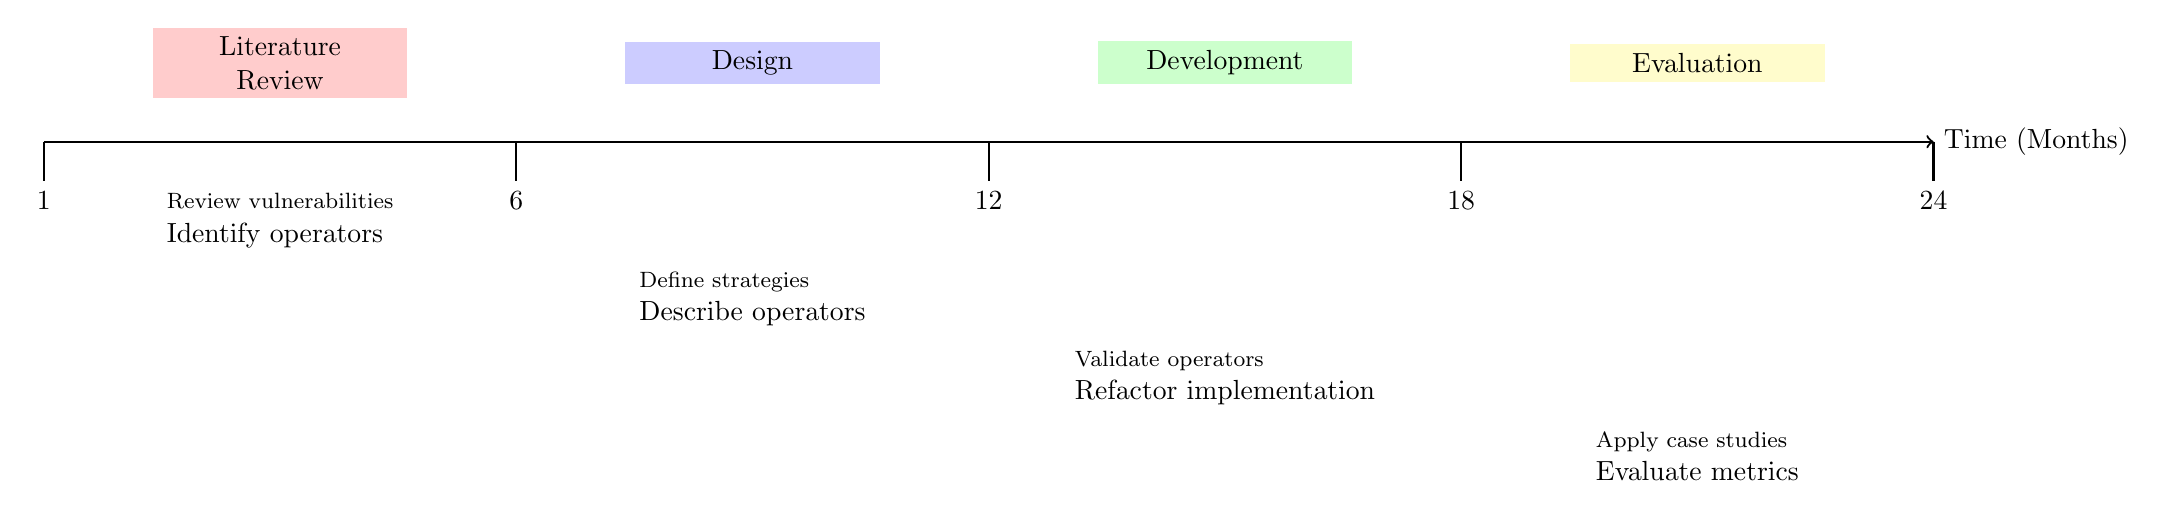
\begin{tikzpicture}
        % Línea de tiempo
        \draw[->, thick] (0,0) -- (24,0) node[right]{Time (Months)};

        % Marcadores de fases
        \draw[thick] (0,0) -- (0,-0.5) node[below]{1};
        \draw[thick] (6,0) -- (6,-0.5) node[below]{6};
        \draw[thick] (12,0) -- (12,-0.5) node[below]{12};
        \draw[thick] (18,0) -- (18,-0.5) node[below]{18};
        \draw[thick] (24,0) -- (24,-0.5) node[below]{24};

        % Fases
        \node[align=center, text width=3cm, fill=red!20] at (3,1) {Literature \\ Review};
        \node[align=center, text width=3cm, fill=blue!20] at (9,1) {Design};
        \node[align=center, text width=3cm, fill=green!20] at (15,1) {Development};
        \node[align=center, text width=3cm, fill=yellow!20] at (21,1) {Evaluation};

        % Notas adicionales
        \node[align=left] at (3,-1) {\footnotesize Review vulnerabilities \\ Identify operators};
        \node[align=left] at (9,-2) {\footnotesize Define strategies \\ Describe operators};
        \node[align=left] at (15,-3) {\footnotesize Validate operators \\ Refactor implementation};
        \node[align=left] at (21,-4) {\footnotesize Apply case studies \\ Evaluate metrics};
    \end{tikzpicture}
  }
    \caption{Timeline of Methodology}
\end{figure}%\includegraphics[width=\textwidth]{timeline_placeholder} % Replace with actual timeline diagram if available.
\end{block}
\end{frame}

\section{Expected Results}


\begin{frame}[allowframebreaks]
\frametitle{Expected Results}
\begin{block}{Impact on RESTful API Security}
\begin{itemize}
    \item Provide a systematic approach for evaluating the robustness of RESTful API security configurations.
    \item Enhance the ability of developers to detect vulnerabilities during the development lifecycle.
\end{itemize}
\end{block}

\begin{block}{Contributions to the Field}
\begin{itemize}
    \item Specification of a comprehensive set of security-aware mutation operators applicable to RESTful APIs.
    \item Introduction of a generic framework for automated security testing tools.
    \item Empirical evidence showcasing improvements in test coverage and fault detection rates.
\end{itemize}
\end{block}

\begin{block}{Anticipated Challenges}
\begin{itemize}
    \item Balancing the trade-off between test coverage and execution time.
    \item Addressing redundancy in mutation operators to avoid excessive equivalent mutants.
    \item Ensuring scalability and applicability across different frameworks and programming languages.
\end{itemize}
\end{block}
\end{frame}

%Print all bibliography
\nocite{*}
\printbibliography[]

\end{document}
